%======================================================================
\chapter{Recommendations}
%======================================================================

Every chapter in a thesis should begin with an introduction and end with a conclusion or a summary.


%----------------------------------------------------------------------
\section{Equations}
% ----------------------------------------------------------------------

In general, equations should be unnumbered unless they referred to in the text. Remember not to leave an empty line before or after the equation in \LaTeX\ because that would start a new paragraph.
%
\begin{equation*}
   \mathcal{R} : \mathbb{R} \to \mathbb{R}^1
\end{equation*}
%
Sometimes, it is better to group related equations together as in~\eqref{eq:trigonometry}. You can refer to subequations as~\eqref{eq:trigonometry:cos}, for example. 
%
\begin{subequations}
  \label{eq:trigonometry}
  \begin{gather}
    \sin^2{\theta} + \cos^2{\theta} = 1  \label{eq:trigonometry:sum}\\
    \cos \theta = \frac{1 - \tan^2(\theta/2)}{1 + \tan^2(\theta/2)}   \label{eq:trigonometry:cos}\\
    \sin \theta = \frac{2 \tan(\theta/2)}{1 + \tan^2(\theta/2)}   \label{eq:trigonometry:sin}
  \end{gather}
\end{subequations}




%----------------------------------------------------------------------
\section{Figures}
% ----------------------------------------------------------------------

\Cref{fig:beam} shows one way of inserting a figure. However, it is sometimes useful to group a few figures together, as in \Cref{fig:experiment1}. For that, it is recommended to use package \texttt{subcaption}. It is preferred to other packages, such as \texttt{subfig}, for instance. Note how you can refer to a subfigure too (e.g.,~\Cref{fig:experiment1:states}).

\begin{figure}[htb]
  \centering
  % 
  \subcaptionbox{Reference/measured vertical acceleration%
    \label{fig:experiment1:ref}}%[12em]%
  {%
    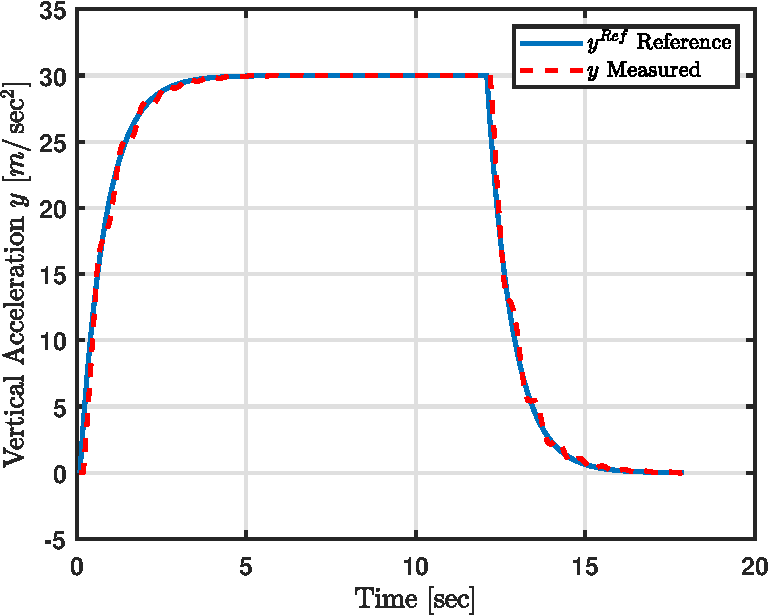
\includegraphics[width=0.32\textwidth]{figures/Matlab/Fig1_1}%
  }
  % 
  \hfill
  %
  \subcaptionbox{Tracking error~$e(t)$%
    \label{fig:experiment1:err}}%[12em]%
  {%
    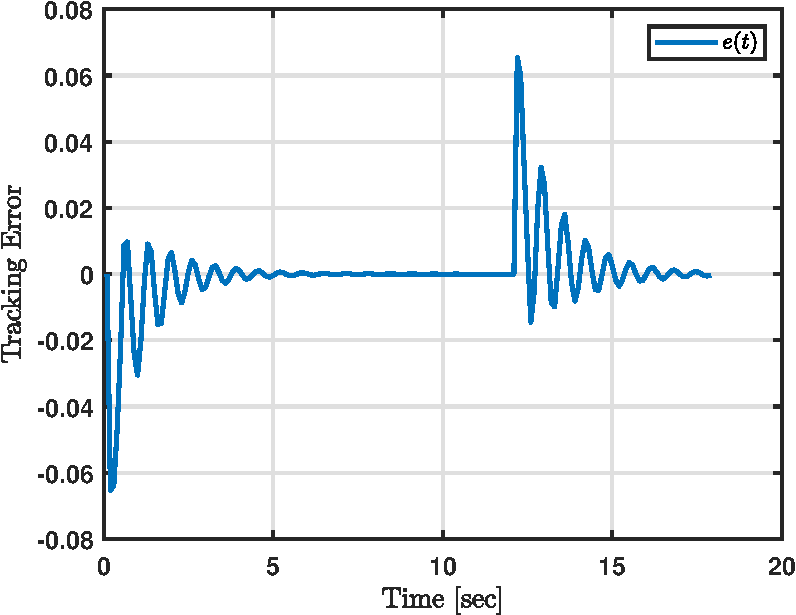
\includegraphics[width=0.32\textwidth]{figures/Matlab/Fig1_5}%
  }
  %
  \hfill
  %
  \subcaptionbox{System states $\alpha(t)$ and~$q(t)$%
    \label{fig:experiment1:states}}%[12em]%
  {%
    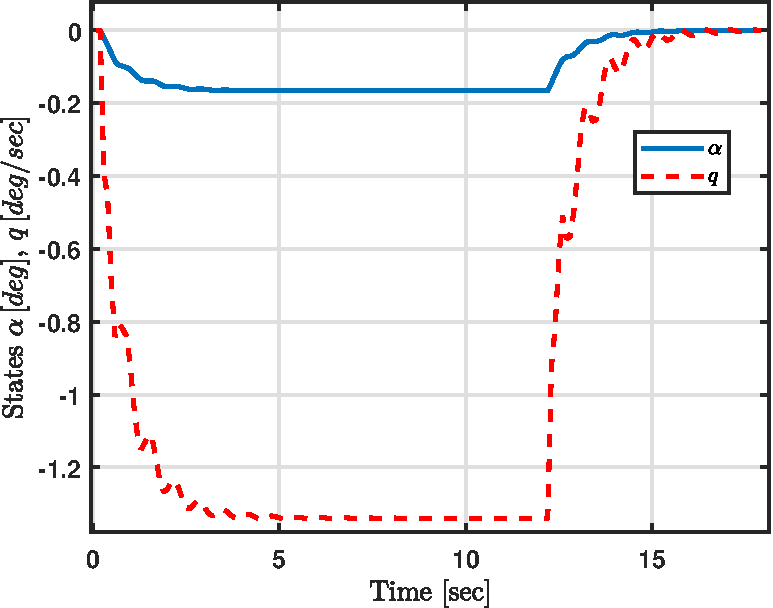
\includegraphics[width=0.32\textwidth]{figures/Matlab/Fig1_2}%
  }
  %
  \\[2ex]
  \mbox{}\hfill
  \subcaptionbox{Elevator deflection~$\bm{u}(t)$%
    \label{fig:experiment1:con}}%[12em]%
  {%
    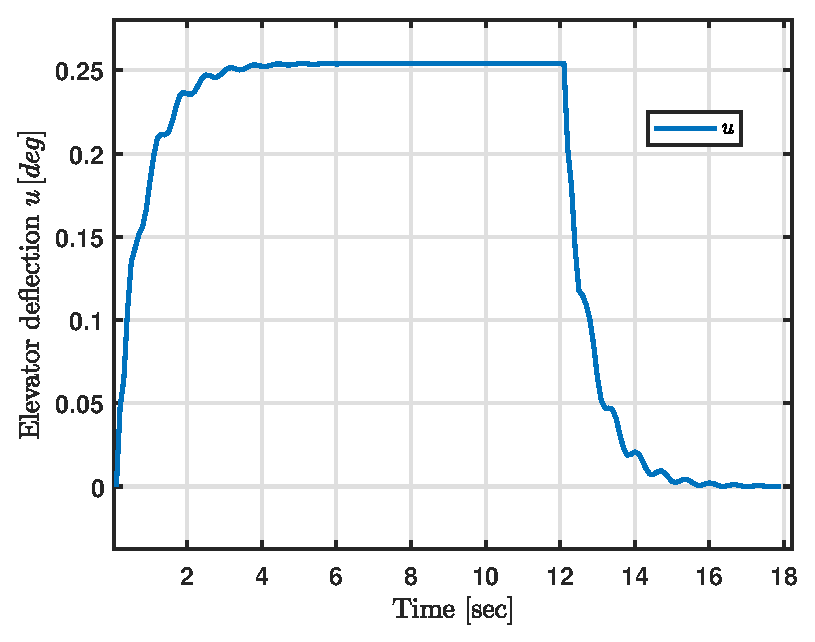
\includegraphics[width=0.32\textwidth]{figures/Matlab/Fig1_3}%
  }
  %
  \hfill
  %
  \subcaptionbox{Control gains~$K(t)$%
    \label{fig:experiment1:act}}%[12em]%
  {%
    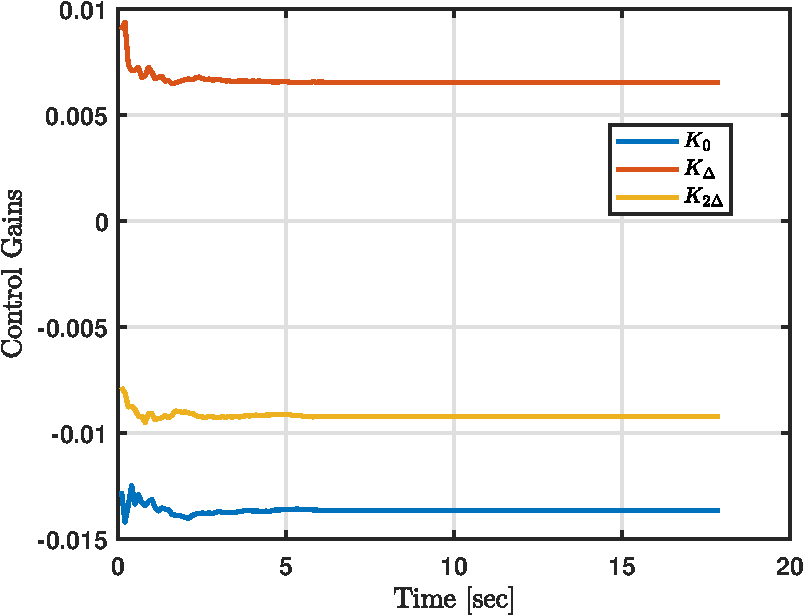
\includegraphics[width=0.32\textwidth]{figures/Matlab/Fig1_4}%
  }
  \hfill\mbox{}
  %
  \caption{Simulation results of test case~1\label{fig:experiment1}} 
\end{figure}





%----------------------------------------------------------------------
\section{Algorithms}
%----------------------------------------------------------------------

\Cref{alg:power} shows an example of how to write algorithms using the \texttt{algorithmicx} package, which is preferred to other packages, such \texttt{algorithmic} and \texttt{algorithm2e}, for example.

\begin{algorithm}[hbt] % or [H]
  \caption{Computing the power of a real number}
  \label{alg:power}
  \begin{algorithmic}[1] % The number tells the line numbering frequency
    \Require
    \Statex $n \geq 0$ \Comment{First input/requirement}
    \Statex $x \in \mathbb{R}$
    \Ensure
    \Statex $y = x^n$
    \Statex % Non-numbered statement
    %
    \State $y \gets 1$
    \State $X \gets x$
    \State $N \gets n$
    \While{$N \neq 0$}
    \If{$N$ is even \algOr $N$ is even}  \Comment{For demonstration purpose}
    \State $X \gets X \times X$
    \State $N \gets \frac{N}{2} $  \Comment{This is a comment}
    \ElsIf{$N$ is odd \algAnd $N$ is odd}
    \State $y \gets y \times X$
    \State $N \gets N - 1$
    \EndIf
    \EndWhile
    %
    \State \Return $y$
  \end{algorithmic}
\end{algorithm}



%----------------------------------------------------------------------
\section{Lists}
%----------------------------------------------------------------------
The default spacing of \LaTeX\ lists can be an eyesore. The package \texttt{enumitem} provides a convenient mechanism to customize them, as illustrated below. Please refer to the package documentation for details.

\begin{itemize}[leftmargin=*, noitemsep]
\item Illum suscipit delenit commodo augue exerci magna veniam hendrerit dignissim duis ut feugait amet dolor dolor suscipit iriure veniam. Vel quis enim vulputate nulla facilisis volutpat vel in, suscipit facilisis dolore ut veniam, duis facilisi wisi nulla aliquip vero praesent nibh molestie consectetuer nulla. Wisi nibh exerci hendrerit consequat, nostrud lobortis ut praesent dignissim tincidunt enim eum accumsan. Lorem, nonummy duis iriure autem feugait praesent, duis, accumsan tation enim facilisi qui te dolore magna velit, iusto esse eu, zzril. Feugiat enim zzril, te vel illum, lobortis ut tation, elit luptatum ipsum, aliquam dolor sed. Ex consectetuer aliquip in, tation delenit dignissim accumsan consequat, vero, et ad eu velit ut duis ea ea odio.
  
\item Vero qui, te praesent et at nisl ut in consequat blandit vel augue ut dolor illum facilisis zzril ipsum. Exerci odio, accumsan ea augue molestie lobortis zzril laoreet ex ad, adipiscing nulla, et dolore, vel te in dolor te, feugait dolore ex vel erat duis. Ut diam commodo ad eu in consequat esse in ut wisi aliquip dolore feugiat wisi eum dignissim tincidunt vel, nostrud. Ut vulputate eum euismod, diam minim eros consequat lorem aliquam et ad luptatum illum sit suscipit ut, tation in dolore euismod et iusto nulla. Iusto wisi odio quis nisl feugiat adipiscing luptatum minim. Illum, quis, erat, dolore qui quis sit dolor veniam blandit ullamcorper ex, vero nonummy, duis exerci delenit ullamcorper at feugiat. Et, ullamcorper elit vulputate iusto esse luptatum duis autem esse nulla qui.

\item Praesent dolore et, delenit, laoreet dolore sed eros hendrerit consequat lobortis. Dolor nulla suscipit delenit commodo augue exerci magna veniam hendrerit dignissim duis ut feugait amet. Ad dolor suscipit iriure veniam blandit quis enim vulputate nulla facilisis volutpat vel in. Erat facilisis dolore ut veniam, duis facilisi wisi nulla aliquip vero praesent nibh molestie consectetuer nulla, iriure nibh exerci hendrerit. Vel, nostrud lobortis ut praesent dignissim tincidunt enim eum accumsan ea, nonummy duis. Ad autem feugait praesent, duis, accumsan tation enim facilisi qui te dolore magna velit, iusto esse eu, zzril vel enim zzril, te. Nisl illum, lobortis ut tation, elit luptatum ipsum, aliquam dolor sed minim consectetuer aliquip.
\end{itemize}

\begin{enumerate}[leftmargin=*, noitemsep]
\item Illum suscipit delenit commodo augue exerci magna veniam hendrerit dignissim duis ut feugait amet dolor dolor suscipit iriure veniam. Vel quis enim vulputate nulla facilisis volutpat vel in, suscipit facilisis dolore ut veniam, duis facilisi wisi nulla aliquip vero praesent nibh molestie consectetuer nulla. Wisi nibh exerci hendrerit consequat, nostrud lobortis ut praesent dignissim tincidunt enim eum accumsan. Lorem, nonummy duis iriure autem feugait praesent, duis, accumsan tation enim facilisi qui te dolore magna velit, iusto esse eu, zzril. Feugiat enim zzril, te vel illum, lobortis ut tation, elit luptatum ipsum, aliquam dolor sed. Ex consectetuer aliquip in, tation delenit dignissim accumsan consequat, vero, et ad eu velit ut duis ea ea odio.
  
\item Vero qui, te praesent et at nisl ut in consequat blandit vel augue ut dolor illum facilisis zzril ipsum. Exerci odio, accumsan ea augue molestie lobortis zzril laoreet ex ad, adipiscing nulla, et dolore, vel te in dolor te, feugait dolore ex vel erat duis. Ut diam commodo ad eu in consequat esse in ut wisi aliquip dolore feugiat wisi eum dignissim tincidunt vel, nostrud. Ut vulputate eum euismod, diam minim eros consequat lorem aliquam et ad luptatum illum sit suscipit ut, tation in dolore euismod et iusto nulla. Iusto wisi odio quis nisl feugiat adipiscing luptatum minim. Illum, quis, erat, dolore qui quis sit dolor veniam blandit ullamcorper ex, vero nonummy, duis exerci delenit ullamcorper at feugiat. Et, ullamcorper elit vulputate iusto esse luptatum duis autem esse nulla qui.

\item Praesent dolore et, delenit, laoreet dolore sed eros hendrerit consequat lobortis. Dolor nulla suscipit delenit commodo augue exerci magna veniam hendrerit dignissim duis ut feugait amet. Ad dolor suscipit iriure veniam blandit quis enim vulputate nulla facilisis volutpat vel in. Erat facilisis dolore ut veniam, duis facilisi wisi nulla aliquip vero praesent nibh molestie consectetuer nulla, iriure nibh exerci hendrerit. Vel, nostrud lobortis ut praesent dignissim tincidunt enim eum accumsan ea, nonummy duis. Ad autem feugait praesent, duis, accumsan tation enim facilisi qui te dolore magna velit, iusto esse eu, zzril vel enim zzril, te. Nisl illum, lobortis ut tation, elit luptatum ipsum, aliquam dolor sed minim consectetuer aliquip.
\end{enumerate}




%----------------------------------------------------------------------
\section{Glossaries}
%----------------------------------------------------------------------
In this template, glossaries are implemented using the package \texttt{glossaries-extra}. Type your glossaries in the file \texttt{glossary.tex}. Either follow the template of the glossary definitions therein or refer to the package documentation.

Here is an example on how to use glossaries. If this is the first time \Gls{FIS} is mentioned in the document, then the full definition is displayed. If it is mentioned again (\Gls{FIS}), then only the abbreviation is shown.




%----------------------------------------------------------------------
\section{Summary}
%----------------------------------------------------------------------
In this chapter, we went through a few recommendations which students may want to keep in mind while typing their theses in \LaTeX. 